\subsection{Simulated Annealing}

\it

Ze względy na ilość uzyskanych wyników porównane zostaną tylko ich średnie wartości.

\rm

\subsubsection{Porównanie parametru spadku temperatury}

\begin{figure}
\begin{center}
\includegraphics[width=0.9\textwidth]{wykresy/sa/sa_200000_av}
\end{center}
\caption{Porównanie różnych spadków temperatury dla temperatury początkowej 200~000.}
\label{sa_200000_av}
\end{figure}

\begin{figure}
\begin{center}
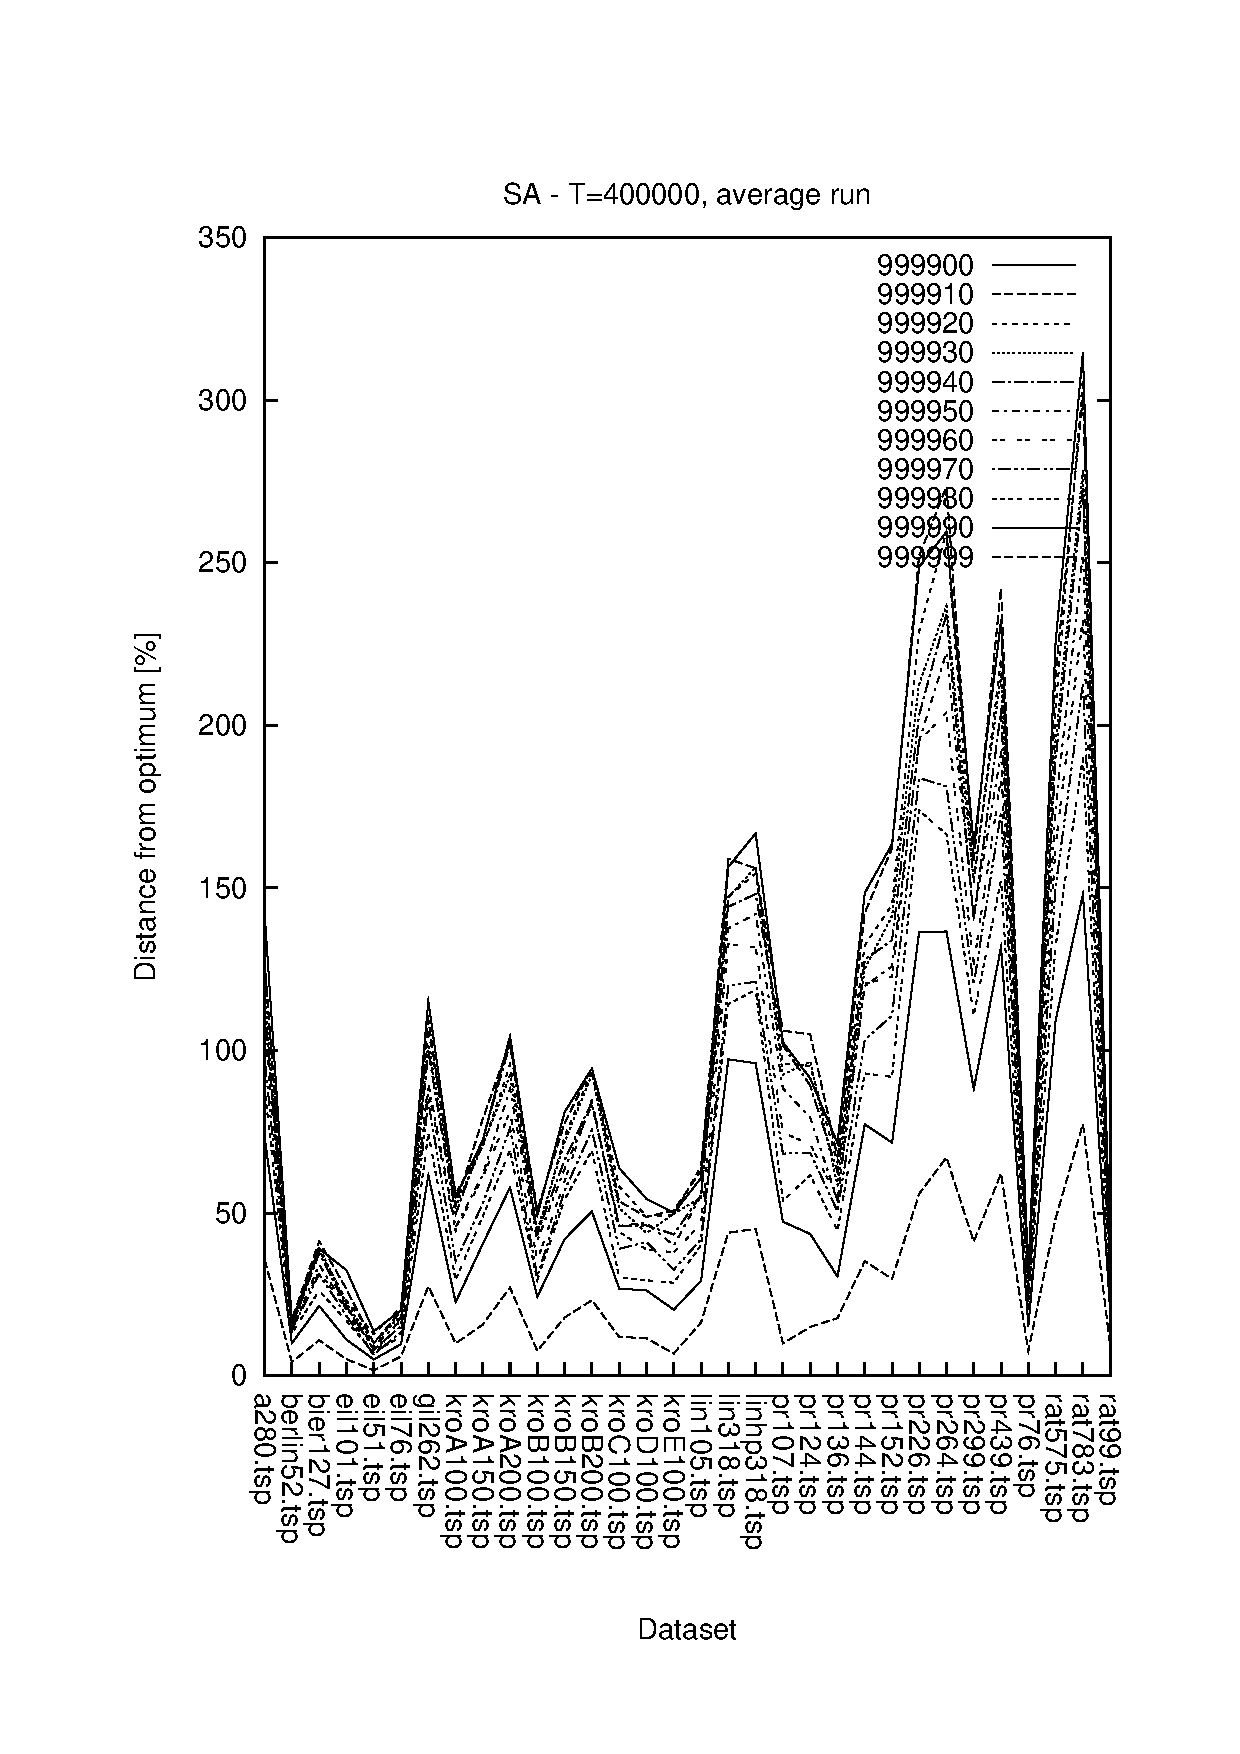
\includegraphics[width=0.9\textwidth]{wykresy/sa/sa_400000_av}
\end{center}
\caption{Porównanie różnych spadków temperatury dla temperatury początkowej 400~000.}
\label{sa_400000_av}
\end{figure}


\begin{figure}
\begin{center}
\includegraphics[width=0.9\textwidth]{wykresy/sa/sa_600000_av}
\end{center}
\caption{Porównanie różnych spadków temperatury dla temperatury początkowej 600~000.}
\label{sa_600000_av}
\end{figure}


\begin{figure}
\begin{center}
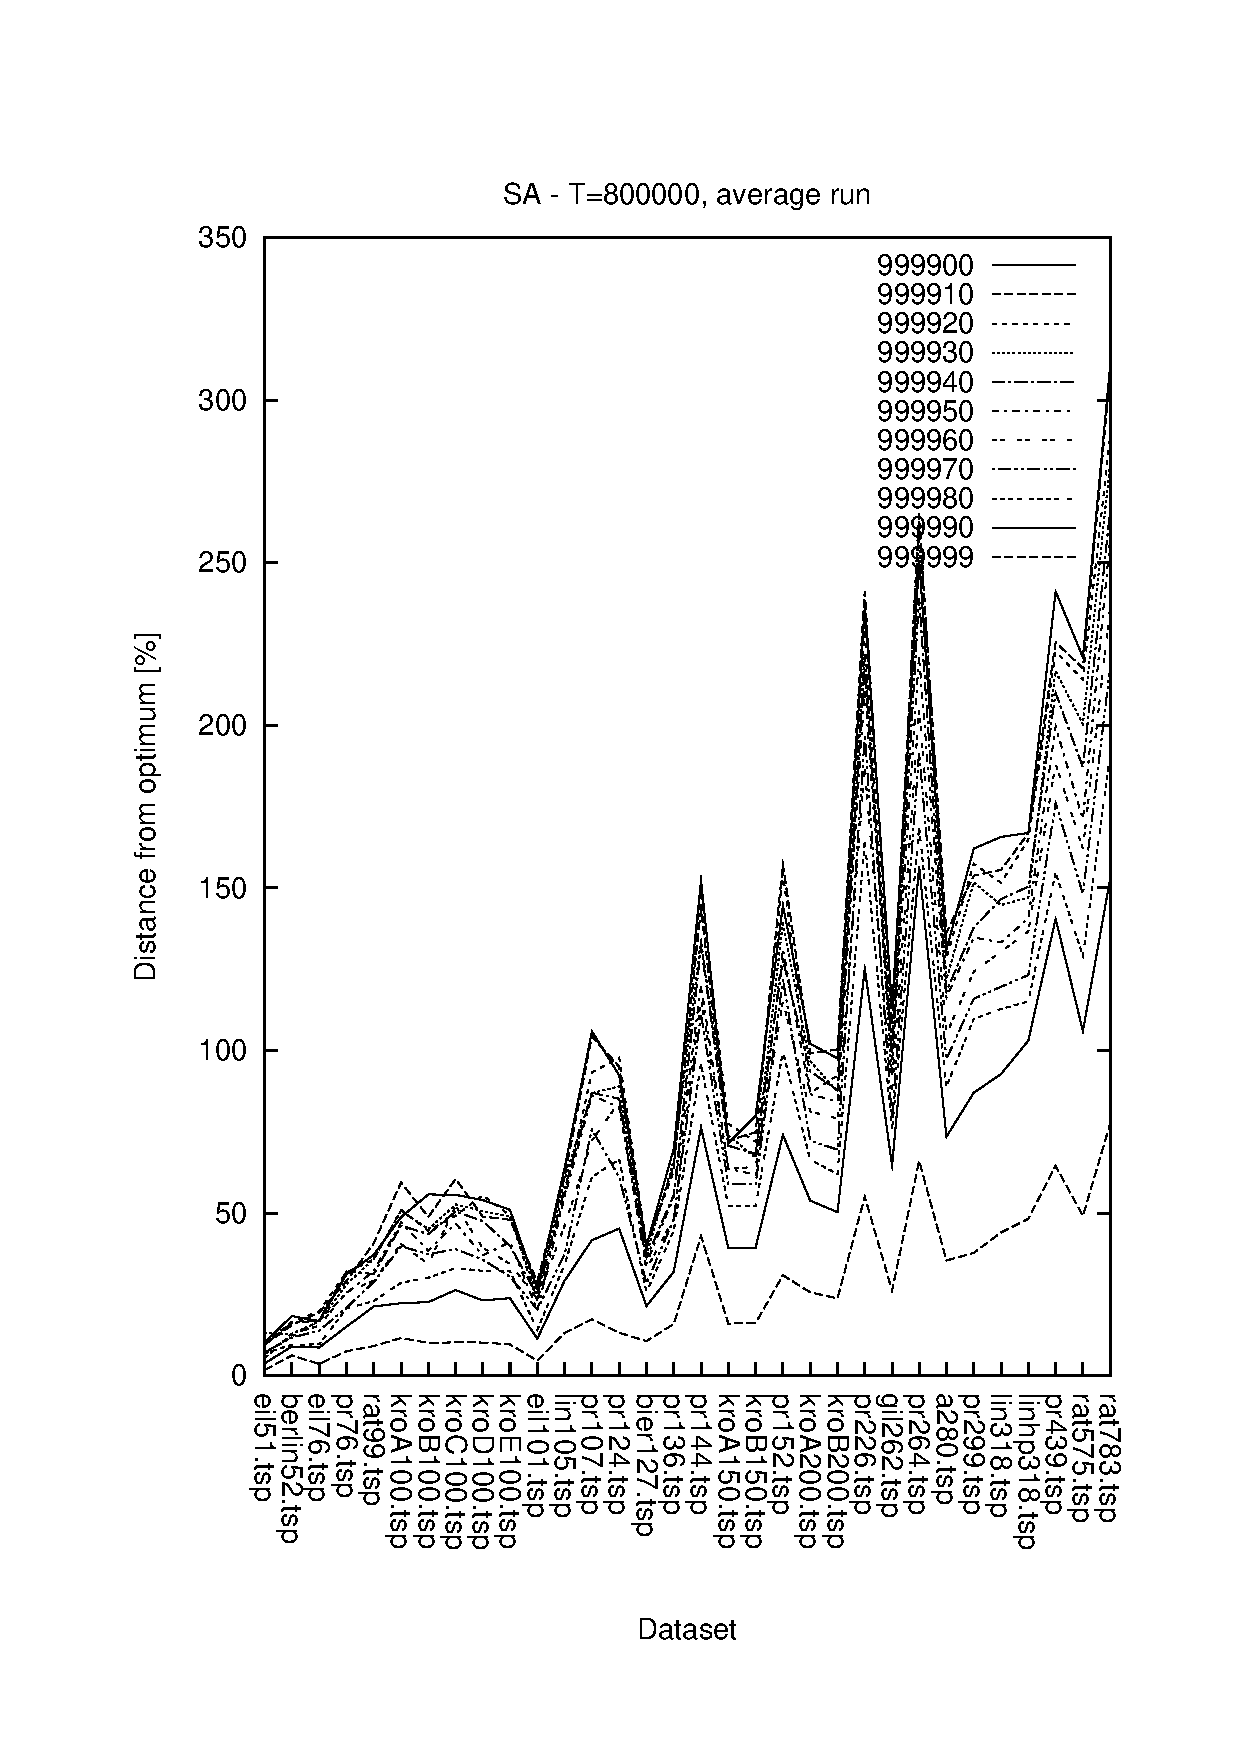
\includegraphics[width=0.9\textwidth]{wykresy/sa/sa_800000_av}
\end{center}
\caption{Porównanie różnych spadków temperatury dla temperatury początkowej 800~000.}
\label{sa_800000_av}
\end{figure}

\begin{figure}
\begin{center}
\includegraphics[width=0.9\textwidth]{wykresy/sa/sa_1200000_av}
\end{center}
\caption{Porównanie różnych spadków temperatury dla temperatury początkowej 1 200~000.}
\label{sa_1200000_av}
\end{figure}


\begin{figure}
\begin{center}
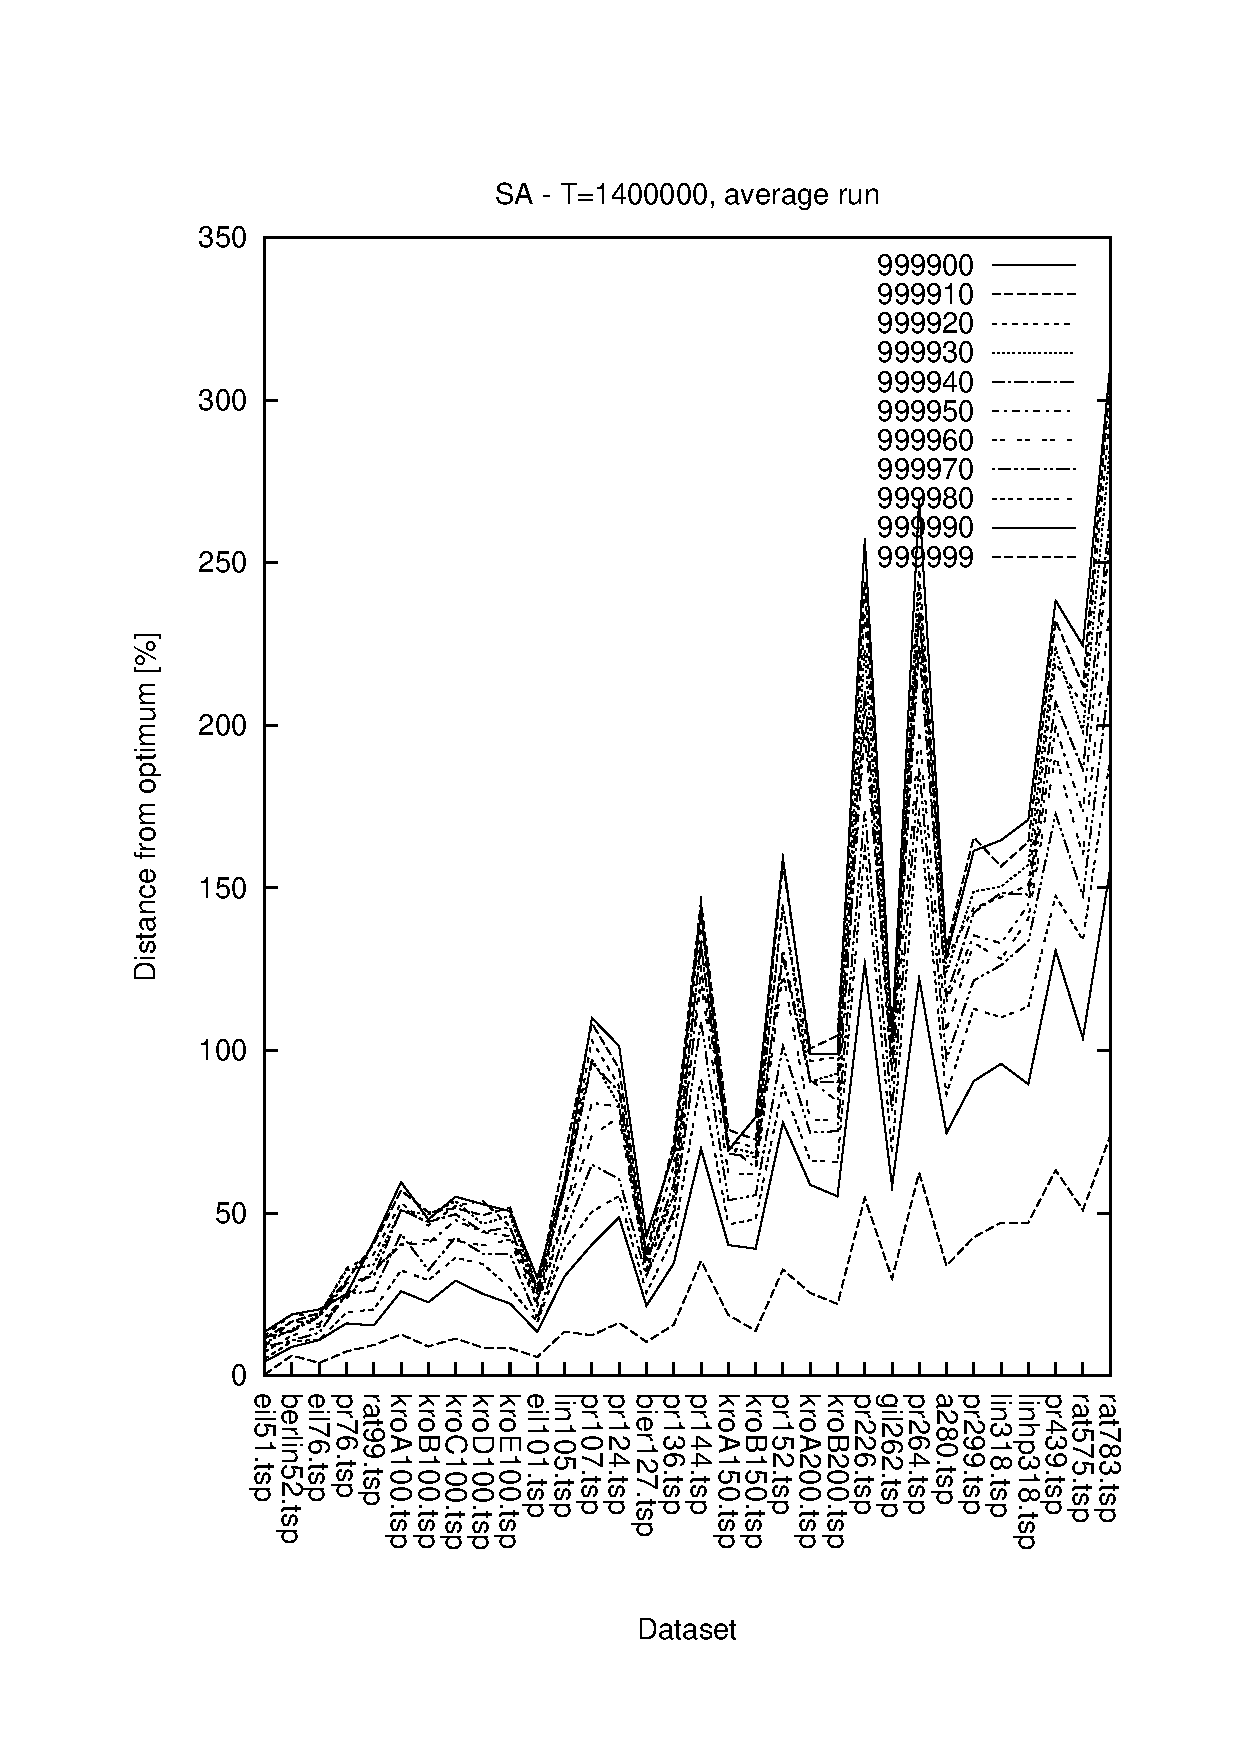
\includegraphics[width=0.9\textwidth]{wykresy/sa/sa_1400000_av}
\end{center}
\caption{Porównanie różnych spadków temperatury dla temperatury początkowej 1 400~000.}
\label{sa_1400000_av}
\end{figure}

\begin{figure}
\begin{center}
\includegraphics[width=0.9\textwidth]{wykresy/sa/sa_1600000_av}
\end{center}
\caption{Porównanie różnych spadków temperatury dla temperatury początkowej 1 600~000.}
\label{sa_1600000_av}
\end{figure}

\begin{figure}
\begin{center}
\includegraphics[width=0.9\textwidth]{wykresy/sa/sa_1800000_av}
\end{center}
\caption{Porównanie różnych spadków temperatury dla temperatury początkowej 1 800~000.}
\label{sa_1800000_av}
\end{figure}

\begin{figure}
\begin{center}
\includegraphics[width=0.9\textwidth]{wykresy/sa/sa_2000000_av}
\end{center}
\caption{Porównanie różnych spadków temperatury dla temperatury początkowej 2 000~000.}
\label{sa_2000000_av}
\end{figure}

\subsubsection{Porównanie parametru temperatury początkowej}

\begin{figure}
\begin{center}
\includegraphics[width=0.9\textwidth]{wykresy/sa_time/99990_Tav}
\end{center}
\caption{Porównanie różnych temperatur początkowych dla spadku temperatury 0,9999.}
\label{999900_Tav}
\end{figure}

\begin{figure}
\begin{center}
\includegraphics[width=0.9\textwidth]{wykresy/sa_time/999920_Tav}
\end{center}
\caption{Porównanie różnych temperatur początkowych dla spadku temperatury 0,99992.}
\label{999920_Tav}
\end{figure}

\begin{figure}
\begin{center}
\includegraphics[width=0.9\textwidth]{wykresy/sa_time/999940_Tav}
\end{center}
\caption{Porównanie różnych temperatur początkowych dla spadku temperatury 0,99994.}
\label{999940_Tav}
\end{figure}

\begin{figure}
\begin{center}
\includegraphics[width=0.9\textwidth]{wykresy/sa_time/999960_Tav}
\end{center}
\caption{Porównanie różnych temperatur początkowych dla spadku temperatury 0,99996.}
\label{999960_Tav}
\end{figure}

\begin{figure}
\begin{center}
\includegraphics[width=0.9\textwidth]{wykresy/sa_time/999980_Tav}
\end{center}
\caption{Porównanie różnych temperatur początkowych dla spadku temperatury 0,99998.}
\label{999980_Tav}
\end{figure}

\begin{figure}
\begin{center}
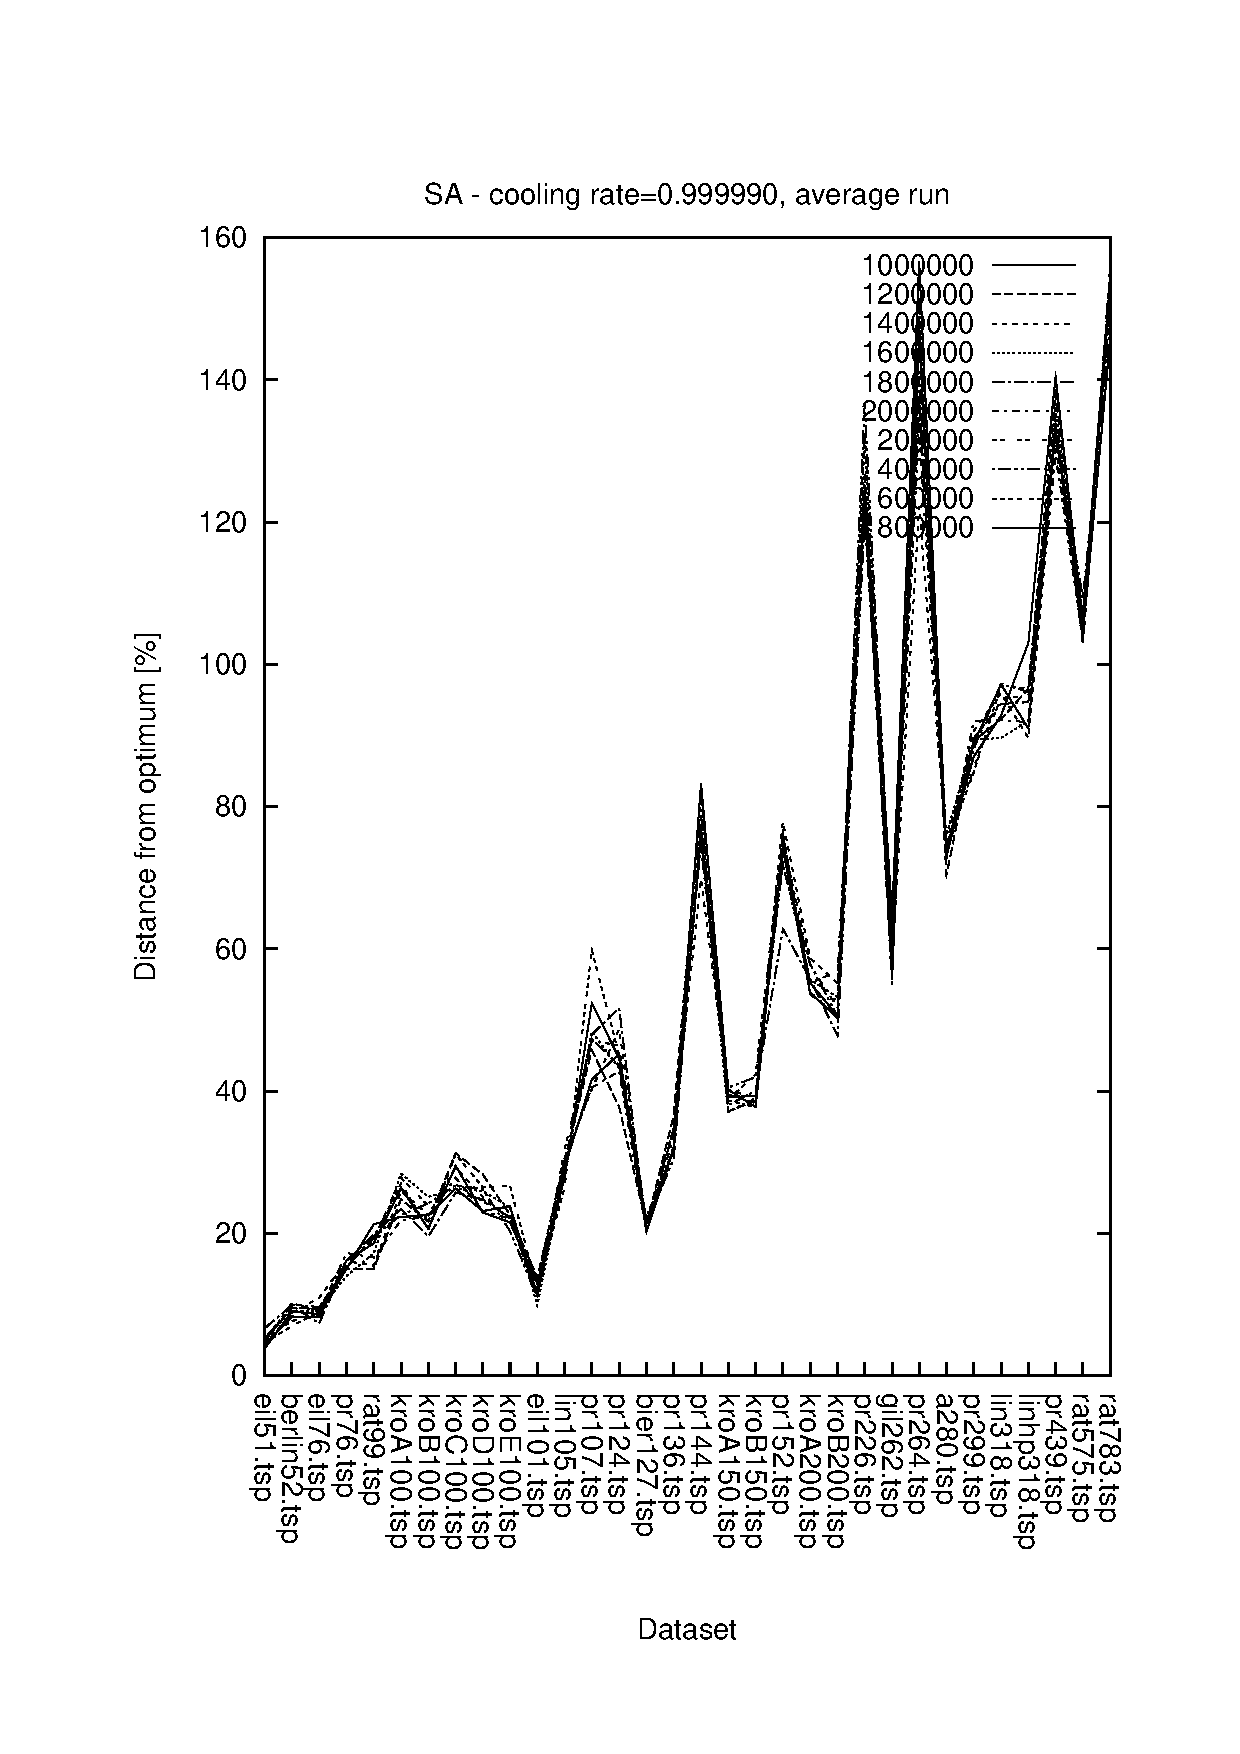
\includegraphics[width=0.9\textwidth]{wykresy/sa_time/999990_Tav}
\end{center}
\caption{Porównanie różnych temperatur początkowych dla spadku temperatury 0,99999.}
\label{999990_Tav}
\end{figure}

\begin{figure}
\begin{center}
\includegraphics[width=0.9\textwidth]{wykresy/sa_time/999999_Tav}
\end{center}
\caption{Porównanie różnych temperatur początkowych dla spadku temperatury 0,999999.}
\label{999999_Tav}
\end{figure}
